The purpose and ambition are to create a \CodeName extension build up on the core API explained in chapter \ref{chp:api}, to demonstrate the opportunities with a tangible and present example to set a standard. The extension seeks to model a data access layer (DAL) as a MapReduce framework (outlined in definition \ref{def:mapreduce}) for \CodeName like Hadoop for HDFS.

\section{Investigation}
The initial idea and thoughts were to create a bridge between the DAL of Disco (described in section \ref{sec:related}) and the API of \CodeName and thereby create a combined integration of the two systems, such that \CodeName would be an optimized and semantic-intelligent replacement for DDFS (Disco Distributed File System). The Disco end-user experience is written in Python programming language like \CodeName and thus would be more convenient to incorporate, rather than frameworks such as Hadoop, which is written in Java.
\newline

The first and foremost reason to design and implement an entirely new framework and thereby discard the Disco based solution was due to the demand and desire to have full control across the whole execution stack from the disk to the end-user input fields. A second and likewise significant reason is the optimization opportunities of having control of the full implementation such as caching of temporary and final results and data accessing.

\section{Assumption}
A small but sufficient number of assumptions has been put together, based on the brief but necessary investigation and the knowledge obtained by the examination of related work in section \ref{sec:related}, to limit the extension to the project scope:

\begin{itemize}
	\item The solution is targeted and used for big data analysis.	
	\item Data is assumed to be research and scientific related material. 
\end{itemize}
, which generally is inspired and based on the ones for \CodeNameShort, listed in section \ref{sec:assumption}.
\newline

Additionally, it is a requirement and thereby an assumption that the \texttt{OperationContext}s (defined in section \ref{sec:operation}) of the datasets can be modeled in terms of a MapReduce scheme.

\section{Objectives} \label{sec:bdae-objectives}
Based on the assumptions and the general knowledge taught by studying similar frameworks has following objectives been composed:
\begin{itemize}
	\item Utilize the \CodeName storage system and its API to create MapReduce based DAL.
	\item Define and design a collection structure to batch similar datasets.
	\item Implement predefined templates for common data structures to reduce redundant tasks for the end-users.
	\item Characterize a domain specific access model.
	\item Load complex data structures such as NetCDF\cite{PageNetCDF} or HDF5\cite{PageHDF5}\cite{Collette:2013:Python} in an intelligent and thus efficiently way to reduce I/O cost.
\end{itemize}

\section{Overview}
BDAE (\textit{/b'dei'/}) is the name and acronym of the big data analysis engine targeting MapReduce operations that are implemented. The solution is built solely using the \CodeName API as illustrated in figure \ref{fig:bdae-overview} and extending existing core components primarily from the foundation package, explained in chapter \ref{chp:components}.

\begin{figure}
	\centering
	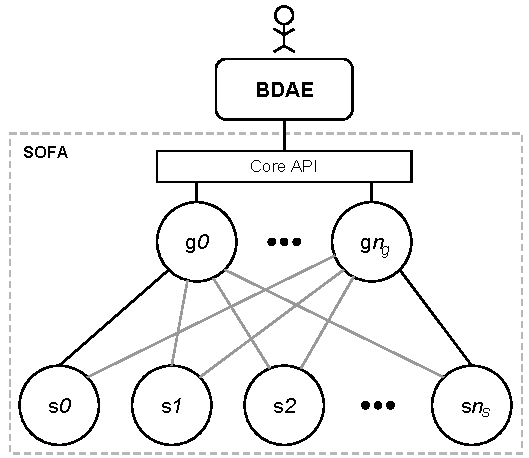
\includegraphics[scale=0.9]{pdf/bdae-overview.pdf}
	\caption[General overview of the BDAE]{General overview of the BDAE integration into \CodeName with same notation as in Figure \ref{fig:sofa-overview}. \label{fig:bdae-overview}}
\end{figure}	


\subsection{Dataset}
The \texttt{SofaBaseObject} defined in section \ref{sec:sofabaseobject} has been extended and delimited along with the requirement of the functions defined in the \texttt{OperationContex}, as a consequence of the chosen execution model. 
\begin{itemize}
	\item A \texttt{MapReduceDataset} has been defined which requires functions executed on the data to be ordered into a \texttt{map} and a \texttt{reduce} category. 
	\item All functions defined in an extended \texttt{OperationContex} is at runtime verified towards the two categories since the MapReduce execution model prescribes that each operation has at least one map function and at most one reduce function as the.
\end{itemize}

\section{Collection} \label{sec:collection}
A dataset in \CodeName is defined by a dictionary with meta data and a list of associated semantic blocks, as previously mentioned in section \ref{sec:sofabaseobject}, but this meta data structure can with slightly modifications also be used as a descriptor for a collection of similar datasets, which was one of the objectives listed in section \ref{sec:bdae-objectives}:

\begin{quotation}
	\textit{"Define and design a collection structure to batch similar datasets."}
\end{quotation}

In other words; a collection in BDAE is defined as a marginally altered meta data dictionary with zero-length list of associated semantic blocks, that nevertheless obeys the interface of the \texttt{SofaBaseObject}, which is a required for any type of data in \CodeName.

\section{MapReduce}
The tree barrier based operation execution model implemented in \CodeName and descried in section \ref{sec:submit} is well-suited for a MapReduce framework and BDAE is utilizing this straightforward advantage. Figure \ref{fig:reduction-tree} illustrates an example of an execution reduction tree as it would resemble with 16 storage nodes, the figure exemplifies among other things how and when the different storage nodes are communicating to calculate the correct result jointly.
\newline

The joints have an important function in the MapReduce framework and have the overall responsibility of why the execution model adds up and it is implemented as following:
\begin{enumerate}
	\item Each node is executing one or more \texttt{map} functions locally.
	\item The neighbor nodes are based on equation \ref{eq:reduction} calculating the locally combined \texttt{reduce} together.
\end{enumerate}

Figure \ref{fig:reduction-tree} illustrates the two steps explained above, where second step is repeated with the same \texttt{reduce} function until all local results are combined to a global result.

\begin{figure}
	\centering
	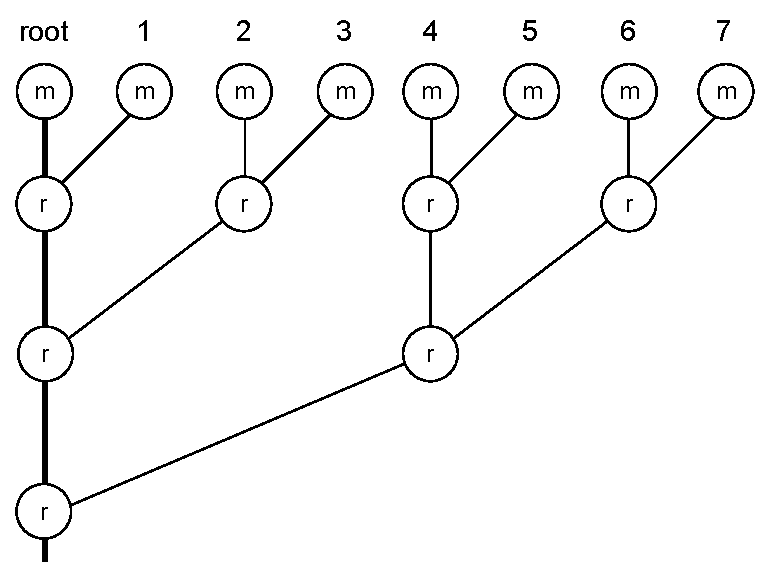
\includegraphics[scale=0.7]{pdf/map-reduce-tree.pdf}
	\caption[BDAE MapReduce implementation]{Utilization of the tree barrier based operation execution model in \CodeName for MapReduce in BDAE. \texttt{m} = map and \texttt{r} = reduce. \label{fig:map-reduce-tree}}
\end{figure}	

\section{User tiers} \label{sec:user-tiers}
One of the objectives for BDAE was to: \textit{"Characterize a domain specific access model"} to first and foremost redeem expectations of system-wide access control, such that the scientist research employees who submit new map reduce operations does not have direct access to boot and teardown servers, as an example.
\newline

The entire BDAE + \CodeName system are divided into three major responsibilities, which each has its domain specific user access level. The responsibilities are inherited as the level increases, which means that a \textbf{manager} have the same rights as the \textbf{scientist} and so fourth.
\newline

The core API of \CodeName has been wrapped into a BDAE specific controller that grants access based on user level, in order to restrict the API access and thus accomplish this.

\subsection{Level 1: Data scientist}
Access rights:
\begin{itemize}
	\item Submit new MapReduce operation
	\item Poll for result
	\item Various \texttt{get}-functions to retrieve meta data information regarding the datasets.
\end{itemize}

\subsection{Level 2: Data manager}
Access rights:
\begin{itemize}
	\item Create dataset
	\item Create collection (essentially a thin wrapper around the create dataset API-call with some extra collection specific logic.)
	\item Append data to dataset
	\item Update/delete dataset
\end{itemize}

\subsection{Level 3: System administrator}
Access rights:
\begin{itemize}
	\item Boot and teardown servers
\end{itemize}

\section{Templates}
BDAE provides a range of different abstract templates related to commonly used data types within the field of interest, to reduce excessive workload for the end-users and generalize the final implementation solution, such that solutions to similar problems are easily comparable.
\newline

\noindent
The templates provided includes:
\begin{itemize}
	\item One for \textbf{text} data that can split raw data into semantic blocks by three different properties: \textit{line}, \textit{sentence} or \textit{word}.
	\item A template for \textbf{image} data that simplifies the burden of transforming raw data such as tiff-files into Numpy arrays.
	\item The template for \textbf{Numpy/Bohrium array}'s is a simple solution that uses the template module binder described subsequently to bind regularly used functions from the respective libraries.
	\item One of the objectives listed in section \ref{sec:bdae-objectives} includes: \textit{"Load complex data structures such as NetCDF $\ldots$ in an intelligent and thus efficiently way to reduce I/O cost."}, which is accomplished by utilizing the collection module described in section \ref{sec:collection} to create a \textbf{NetCDF} template. This is possible since this data format essentially is a group of related data records. 
\end{itemize}

\subsection{Module binder}
The module binder is not as such a template, but provides opportunities for conveniently binding Python built-in and other third party library functions like \texttt{map} and \texttt{reduce} specific \texttt{OperationContext} functions.
\newline

An example: \texttt{count(}x, y\texttt{)} is a built-in function from the \texttt{string} module in Python \cite{PagePython} that counts number of \texttt{y} in \texttt{x}. The following snippet transforms the \texttt{count(}x, y\texttt{)} into \texttt{count\_occurrences(}x, y\texttt{)} with identical logic parameters and results.
\vspace*{2mm}
\begin{lstlisting}[language=Python, basicstyle=\footnotesize, numbers=none, showtabs=false, showstringspaces=false, showspaces=false, otherkeywords={string,new_fun_names}, stringstyle=\color{blue}]
   module_binder(string, function_binder, ['count'], 
                 new_fun_names=['count_occurrences'])
\end{lstlisting}
\vspace*{-6mm}

\section{Libraries}
BDAE provides three python libraries one for each of the user tier described in section \ref{sec:user-tiers}: \texttt{libbdaescientist}, \texttt{libbdaemanager} and \texttt{libbdaeadmin} respectively.

\subsection{Web}
\subsection{Android App} \label{sec:bdaeapp}